\documentclass{beamer}


\usetheme{simple}

\usepackage{lmodern}
\usepackage[scale=2]{ccicons}

\usepackage[margin=1cm]{caption}

\usepackage[linesnumbered, ruled]{algorithm2e}
\usepackage{subcaption}
\usepackage{graphicx}
\usepackage[T2A]{fontenc} % enable Cyrillic fonts
\usepackage[english,serbian]{babel}


% TODO: 
%   position adjustement
%   change colours
%       

% Watermark background (simple theme)

\setwatermark{
\includegraphics[height=8cm]{matf_logo1.png}}


\title{Memetski algoritam i njegove primene}
\subtitle{}
\date{\today}
\author{Marica Bogićević, Boris Karanović, Petar Košanin, Filip Šašić}
\institute{Matematički Fakultet}

\begin{document}

\maketitle




%%% Uvod %%%
\begin{frame}[fragile]{Uvod}
  \framesubtitle{Opšti memetski algoritam}
  
   \begin{itemize}
    \item{Generiši početnu populaciju}
    \item{Dokle god nije ispunjen uslov zaustavljanja}
        \begin{itemize}
             \item{Evaluiraj sve jedinke u populaciji}
             \item{Selektuj jedinke za ukrštanje}
             \item{Izvrši ukrštanje i mutaciju}
             \item{Za svaku novu jedinku}
                \begin{itemize}
                     \item{Izvrši učenje pojedinačne jedinke na odabrani način}
                \end{itemize}
        \end{itemize}
          \item{Kraj algoritma}

  \end{itemize}

\end{frame}
%%% ---- %%%%

\begin{frame}[fragile]{Problem trgovačkog putnika}
  \framesubtitle{Memetski algoritam i njegove primene}
  
   \begin{itemize}
    \item{NP težak problem, složenosti O(n!)}
    \item{1932. - Karl Menger definisao pojam ''trgovački putnik'' }
     \item{Nestandardne karakteristike lokalne pretrage:}
        \begin{itemize}
             \item{Navođena lokalna pretraga\cite{Memetic}}
             \item{Lokalan pretraga sa više početaka}
        \end{itemize}
     \item{Standardna lokalna pretraga se najbolje pokazala}
  \end{itemize}

\end{frame}


\begin{frame}[fragile]{Problem trgovačkog putnika}
  \framesubtitle{Memetski algoritam i njegove primene}
  
   \begin{itemize}
    \item{Standardna lokalna pretraga primenjena na roditelje sa verovatnoćom Pls}
  \begin{itemize}
    \item{indip = getIterator(Parents);}
     
    \item{If (($Pls \geqslant	 rand(0,1)) \wedge indip \neg best solution$)}
    \item{Apply\_Move(indip);}
     \begin{itemize}
       \item{Modify(indip);}
        \item{If(prevFitness < newFitness)}
        \item{If(random(0,1) > treshold)}
        \item{Accept;}
        \end{itemize}
   \end{itemize}
  \end{itemize}

\end{frame}

\begin{frame}[fragile]{Problem trgovačkog putnika}
  \framesubtitle{Memetski algoritam i njegove primene}

    \begin{itemize}
     \item{Modify(indip)}
       \begin{itemize}
     \item{2swap pomeranje}
     \end{itemize}
   
  
    \item{Select\_mating(Parents)}
     \begin{itemize}
     \item{Turnirska selekcija}
     \end{itemize}
       \item{Ukrštanje}
       \begin{itemize}
     \item{Jednopoziciono}
     \end{itemize}
     
     \item{Mutacija}
      \begin{itemize}
     \item{jedinka može mutirati više puta u cilju opstanka}
     \end{itemize}
   \item{Select\_Parents(Parents,Offsprings)}
      \begin{itemize}
     \item{$(\mu + \lambda)$ ili $(\mu,\lambda)$ strategija\cite{MuLambda}}
     \end{itemize}
  \end{itemize}

\end{frame}

\begin{frame}[fragile]{Detektovanje zajednica}
  \framesubtitle{Memetski algoritam i njegove primene}
 
  \begin{itemize}
   \item 
   Ima za cilj pronalazak  podskupa čvorova grafa čiji je skup međusobnih grana gušći nego ostatak grafa.
    \end{itemize}
    
    
      \begin{itemize}
   \item Primena u marketingu, trgovini, društvenim mrežama...
    \end{itemize}
    
    \begin{itemize}
   \item Koristi gustinu modularnosti kao meru kvaliteta umesto modularnosti
    \end{itemize}
    \end{frame}
    
\begin{frame}[fragile]{Detektovanje zajednica}
  \framesubtitle{Memetski algoritam i njegove primene}
    Algoritam ima sledeću formu:
    
       \begin{itemize}
   \item{Kodiranje jedinki}
        \begin{itemize}
             \item Jednu jedinku populacije čini niz celih brojeva: $X = [x_1, x_2,...,x_n]$, gde je $n$ ukupan broj čvorova mreže
    \end{itemize}
    \item{Inicijalizacija populacije}
    \item{Lokalna pretraga}
    \begin{itemize}
        \item maksimizuje gustinu modularnosti, kreće od suseda do suseda u prostoru kandidata pretrage
    \end{itemize}
    \item{Selekcija}
        \begin{itemize}
        \item Turnirska selekcija
    \end{itemize}
    \item{Operator ukrštanja}
        \begin{itemize}
            \item Dvopoziciono ukrštanje
        \end{itemize}

  \end{itemize}

\end{frame}


\begin{frame}[fragile]{Detektovanje zajednica}
  \framesubtitle{Memetski algoritam i njegove primene}
  
    \begin{figure}[h!]
     	\centering
     	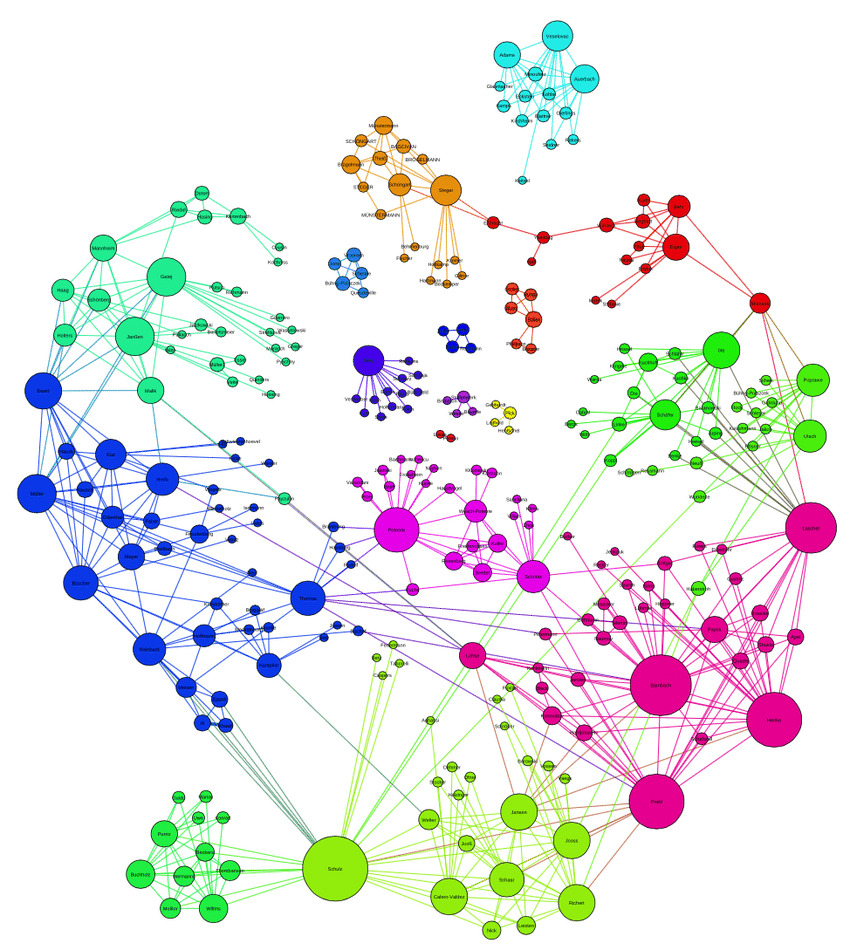
\includegraphics[scale=0.2]{gnn.jpg}
        \caption{Primer detektovanja zajednica. Izvor \cite{comd}}
    \end{figure}
  
\end{frame}

\begin{frame}[fragile]{Bojenje grafa}
  \framesubtitle{Memetski algoritam i njegove primene}
    \begin{figure}[h!]
     	\centering
     	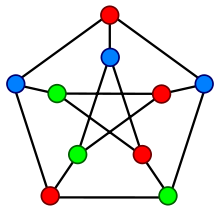
\includegraphics[scale=0.5]{bojene_grafa1}
        \caption{Primer ispravnog bojenja čvorova grafa. Izvor \cite{graph_coloring}}
    \end{figure}
    
    \begin{itemize}
        \item NP-kompletan problem
        \item Nalazi razne praktične primene kao npr. alokacija registara
    \end{itemize}
\end{frame}



\begin{frame}[fragile]{Bojenje grafa}
  \framesubtitle{Memetski algoritam i njegove primene}

Neka je zadat neusmern graf $G = (V, E)$

   \begin{itemize}
    \item{Hibridni algoritam za bojenje(HCA)}
        \begin{itemize}
            \item Jednu jedinku populacije čini podela skupa $V$ na $k$  disjunktnih podskupova $\{V_1, V_2, ...., V_k\}$
            \item Tabu pretraga
            \item GPX operator ukrštanja \cite{galinier1999hybrid}
        \end{itemize}
    \item{Memetski algoritam za bojenje grafa(MACOL)}
        \begin{itemize}
            \item Više od dve jedinke učestvuje u operatoru ukrštanja
        \end{itemize}
    \item{Hibridni evolutivni algoritam u duetu(HEAD)}
        \begin{itemize}
            \item Dve jedinke čine populaciju
            \item Najbolja rešenja učestvuju u ukrštanju
        \end{itemize}
  \end{itemize}
  

\end{frame}




%%% Zaključak %%%
\begin{frame}[fragile]{Zaključak}
  
   \begin{itemize}
    \item{Memetski algoritam pronalazi primene u raznoraznim realnim i naučnim problemima}
    \item{U zavisnosti od izabranih parametara, može davati dosta bolje rezultate od prostog genetskog algoritma}
    \item{Veoma je bitno koliko vremena treba posvetiti metodi koja lokalno optimizuje jedinku}
    
    \end{itemize}
\end{frame}
%%% ---- %%%%


\begin{frame}{Kraj}
  \framesubtitle{Memetski algoritam i njegove primene}

  
\centering
\Huge{Hvala na pažnji!}

\end{frame}




\begin{frame}{Kraj}
  \framesubtitle{Memetski algoritam i njegove primene}
\centering
\Huge{Pitanja?}

\end{frame}

\bibliography{references.bib} 
\bibliographystyle{plain}




\end{document}